\documentclass{article}
\usepackage{geometry}
\usepackage{graphicx}
\graphicspath{ {./imgs/} }
\usepackage{circuitikz}
\usepackage{siunitx}

\geometry{margin=1in}
\author{Ty Davis}
\title{Lab 3 Report}
\newcommand{\twopics}[4]{
\begin{figure}
\begin{center}
  \begin{minipage}{.45\textwidth}
    \includegraphics[width=\textwidth]{#1}
  \end{minipage}
  \begin{minipage}{.45\textwidth}
    \includegraphics[width=\textwidth]{#2}
  \end{minipage}
  \label{#3}
  \caption{#4}
\end{center}
\end{figure}
}

\begin{document}
\maketitle

\section{Circuit A - The Limiter Circuit}

This first circuit is a limiter, which means that it
limits the output of the circuit so that the maximums
and minimums of the peaks are a little bit lower than
they were before.

\begin{figure}[h!]
  \centering
  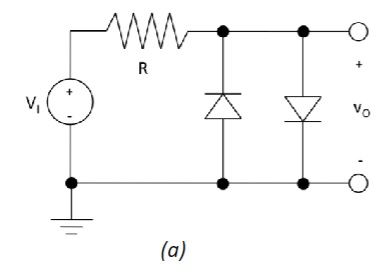
\includegraphics{imgs/circuits/circuita.jpg}
  \label{circuita}
\end{figure}

The circuit in Figure (A) is the limiter
circuit that we built in the first lab. The resistor
we used was a 10~k$\Omega$ resistor, measured at
9.998~k$\Omega$. When supplied with an input voltage
of 5 V$_{pk-pk}$ we saw that the output voltage 
was decreases slightly both in our measured circuit 
and in the simulation. In Figure \ref{circuitalinear} 
we can see that the voltage of the output is reduced
to just 1.41 V$_{pk-pk}$.

\twopics{imgs/scope/scope_CircuitA}{imgs/sim/Circuit A}{circuitalinear}{Measured and Simulated Results for Circuit A}

Those voltages are shown in X-Y mode in Figure \ref{circuitaxy}.

\twopics{imgs/scope/scope_CircuitA_XY}{imgs/sim/Circuit A X-Y}{circuitaxy}{Measured and Simulated Results for Circuit A in XY Mode}


\pagebreak
\section{Circuit B - The Zener Limiter Circuit}
This is similar to the first circuit but it uses 
Zener diodes which operate in the breakdown voltage
as their function.


\begin{figure}[h!]
  \centering
  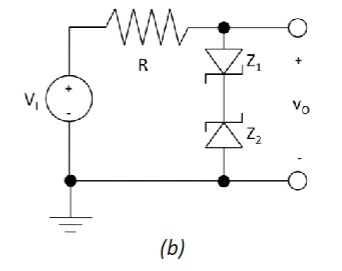
\includegraphics{imgs/circuits/circuitb.jpg}
  \label{circuitb}
\end{figure}

The circuit in Figure (B) is the Zenode limiter
circuit that we built in the first lab. The resistor
we used was a 1~k$\Omega$ resistor, measured at
1.003~k$\Omega$. When supplied with an input voltage
of 15 V$_{pk-pk}$ we saw that the output voltage 
was decreases slightly both in our measured circuit 
and in the simulation. In Figure \ref{circuitblinear} 
we can see that the voltage of the output is reduced
to just 12.9 V$_{pk-pk}$.

It wasn't reduced as much as in the first circuit,
but there was still a reduction when the voltage got 
close to its peak.

\twopics{imgs/scope/scope_CircuitB}{imgs/sim/Circuit B}{circuitblinear}{Measured and Simulated Results for Circuit B}

Those voltages are shown in X-Y mode in Figure \ref{circuitbxy}.

\twopics{imgs/scope/scope_CircuitB_XY}{imgs/sim/Circuit B X-Y}{circuitbxy}{Measured and Simulated Results for Circuit B in XY Mode}


\pagebreak

\section{Circuit C - The Clamped Capacitor Circuit}


\begin{figure}[h!]
  \centering
  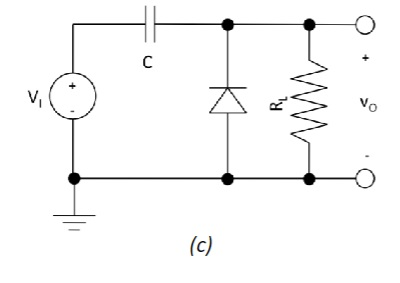
\includegraphics{imgs/circuits/circuitc.jpg}
  \label{circuitc}
\end{figure}

The circuit in Figure (C) is the Clamped Capacitor
circuit that we built in the first lab. 
We fed it with a 2 V$_{pk-pk}$ square wave and it 
resulted in the output shown in Figure \ref{circuitclinear}

In these images the values are a little skewed, but the
output voltage as a 2 V$_{pk-pk}$ square wave but with a 
DC Offset of about $+ 1$ V.

\twopics{imgs/scope/scope_CircuitC}{imgs/sim/Circuit C}{circuitclinear}{Measured and Simulated Results for Circuit C}

\pagebreak
\section{Circuit D - The Voltage Doubler Circuit}


\begin{figure}[h!]
  \centering
  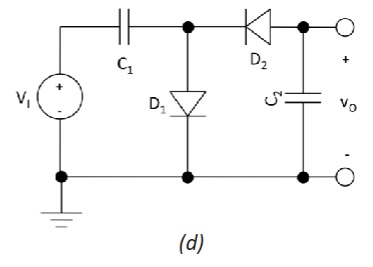
\includegraphics{imgs/circuits/circuitd.jpg}
  \label{circuitd}
\end{figure}

The circuit in Figure (D) is the Voltage Doubler
circuit that we built in the first lab. 
We fed it with a 5 V$_{pk-pk}$ sine wave and it 
resulted in the output shown in Figure \ref{circuitdlinear}

The resulting voltage on the output is a constant DC 
voltage but the output is two times higher than the 
lowest value provided in the sine wave. So it not
only converts the AC voltage to DC, but also doubles the
DC value as the minimum value reached was -4.42 V, and 
the lowest value from the input was -2.5 V.

\twopics{imgs/scope/scope_CircuitD}{imgs/sim/Circuit D}{circuitdlinear}{Measured and Simulated Results for Circuit D}


\pagebreak
\section{Conclusion}
Using diodes and capacitors you can make a variety of 
different circuits to achieve different results on the
output voltages. I thought the most interesting circuits
were circuits C and D because they had the most 
interesting affects on the input voltages.

\end{document}